\documentclass[11pt,a4paper]{article}
\usepackage[utf8]{inputenc}
\usepackage[brazil]{babel}
\usepackage{amsmath,amssymb}
\usepackage{graphicx}
\usepackage{booktabs}
\usepackage{listings}
\usepackage{xcolor}
\usepackage{geometry}
\usepackage{hyperref}
\usepackage{caption}

\geometry{top=2.5cm, bottom=2.5cm, left=2.5cm, right=2.5cm}

\definecolor{codegreen}{rgb}{0,0.6,0}
\definecolor{codegray}{rgb}{0.5,0.5,0.5}
\definecolor{codepurple}{rgb}{0.58,0,0.82}
\definecolor{backcolour}{rgb}{0.96,0.96,0.96}

\lstdefinestyle{pythonstyle}{
    backgroundcolor=\color{backcolour},   
    commentstyle=\color{codegreen},
    keywordstyle=\color{blue}\bfseries,
    numberstyle=\tiny\color{codegray},
    stringstyle=\color{codepurple},
    basicstyle=\ttfamily\footnotesize,
    breakatwhitespace=false,         
    breaklines=true,                 
    captionpos=b,                    
    keepspaces=true,                 
    numbers=left,                    
    numbersep=5pt,                  
    showspaces=false,                
    showstringspaces=false,
    showtabs=false,                  
    tabsize=4,
    frame=single
}

\lstset{style=pythonstyle}

\title{\textbf{Relat\'{o}rio T\'{e}cnico -- Cr\'{e}dito 2}\\\large Implementa\c{c}\~{a}o do FCM e Obten\c{c}\~{a}o Emp\'{i}rica da Fun\c{c}\~{a}o Tempo\\\textbf{Equipe 06 -- Miss\~{a}o 6: Loop Fission (Div\'{o}rcio de La\c{c}os)}}
\author{
    \textbf{Caio Lopes Da Silva} (Matr\'{i}cula: 072410052) \\
    \textbf{Ma Qi Chao} (Matr\'{i}cula: 072410078) \\
    \textbf{Lucian Vitor Silva Nascimento} (Matr\'{i}cula: 072410137) \\
    \vspace{0.2cm}\\
    Universidade do Estado da Bahia (UNEB) -- DCET I \\
    Disciplina: Engenharia de Programas \\
    Prof. Dr. Diego Gervasio Frias Suarez
}
\date{28 de outubro de 2026}

\begin{document}

\maketitle

\section{Introdu\c{c}\~{a}o e Escopo}
Este documento apresenta os resultados formais do Cr\'{e}dito 2 da disciplina de Engenharia de Programas. O objetivo central consiste em descrever a implementa\c{c}\~{a}o autoral e rigorosa \textit{from scratch} do algoritmo de agrupamento difuso \textit{Fuzzy C-Means} (FCM), respeitando estritamente a restri\c{c}\~{a}o arquitetural sorteada para a nossa equipe, bem como apresentar a modelagem matem\'{a}tica do Tempo Emp\'{i}rico de execu\c{c}\~{a}o ($T_{\text{exp}}$) em fun\c{c}\~{a}o da dimensionalidade da imagem de entrada ($n$ pixels) e do n\'{u}mero de agrupamentos ($K$ \textit{clusters}), seguindo os preceitos metodol\'{o}gicos do Protocolo F.O.C.A.

\section{An\'{a}lise da Restri\c{c}\~{a}o Arquitetural}
\textbf{Restri\c{c}\~{a}o Sorteada: Miss\~{a}o 6 -- Loop Fission (Div\'{o}rcio de La\c{c}os)}

A transforma\c{c}\~{a}o de \textit{Loop Fission} (ou distribui\c{c}\~{a}o de la\c{c}os) \'{e} uma t\'{e}cnica cl\'{a}ssica da teoria de compiladores e otimiza\c{c}\~{a}o de c\'{o}digo em que um la\c{c}o \'{u}nico com m\'{u}ltiplas instru\c{c}\~{o}es \'{e} cindido em dois ou mais la\c{c}os independentes que iteram sobre o mesmo espa\c{c}o de \'{i}ndices.

Do ponto de vista da microarquitetura e da hierarquia de mem\'{o}ria:
\begin{itemize}
    \item \textbf{Destrui\c{c}\~{a}o da Localidade Temporal de Cache (L1/L2):} No c\'{o}digo basal (\textit{Baseline}), as dist\^{a}ncias euclidianas calculadas para um pixel s\~{a}o imediatamente consumidas na linha subsequente para o c\'{a}lculo da pertin\^{e}ncia fuzzy. Esses dados permanecem quentes nos registradores da CPU ou na mem\'{o}ria Cache L1 (lat\^{e}ncia de $\approx 1$ ns). Com o \textit{Loop Fission}, a separa\c{c}\~{a}o dos la\c{c}os for\c{c}a o armazenamento de todas as dist\^{a}ncias em uma matriz intermedi\'{a}ria de ordem $n \times K$. Ao terminar o primeiro la\c{c}o sobre dezenas de milhares de pixels, a capacidade volum\'{e}trica das caches L1 e L2 \'{e} completamente esgotada (\textit{cache eviction}). Quando o segundo la\c{c}o inicia a leitura dos primeiros elementos, a CPU sofre \textit{cache misses} massivos, sendo compelida a requisitar dados diretamente da mem\'{o}ria RAM principal (lat\^{e}ncia de 50 a 100 ns).
    \item \textbf{Sobrecarga de Aloca\c{c}\~{a}o Din\^{a}mica e Controle:} A cis\~{a}o duplica o n\'{u}mero de desvios condicionais (\textit{branches} de la\c{c}o) e imp\~{o}e ao interpretador a aloca\c{c}\~{a}o din\^{a}mica cont\'{i}nua de centenas de milhares de objetos \texttt{PyListObject} no \textit{heap}, ativando ciclos recorrentes de coleta de lixo (\textit{garbage collection}).
\end{itemize}

\section{Implementa\c{c}\~{a}o do N\'{u}cleo FCM}
O c\'{o}digo-fonte completo, contendo os scripts de valida\c{c}\~{a}o, o harness experimental e os artefatos de bancada, encontra-se versionado no seguinte reposit\'{o}rio p\'{u}blico:

\noindent\textbf{Link do Reposit\'{o}rio:} \url{https://github.com/MaQiChao1308/Engenharia-de-Programas}

Abaixo, destaca-se o \textit{snippet} da a\c{c}\~{a}o cir\'{u}rgica executada pela Equipe 6 sobre o la\c{c}o principal do FCM, demonstrando o div\'{o}rcio estrutural entre a fase de c\'{a}lculo de dist\^{a}ncias e a fase de atualiza\c{c}\~{a}o da matriz de pertin\^{e}ncia e converg\^{e}ncia.

\begin{lstlisting}[language=Python, caption={N\'{u}cleo computacional do FCM com Loop Fission (Miss\~{a}o 6).}]
# ====================================================================
# EXECUCAO CIRURGICA: MISSAO 6 (Loop Fission / Divorcio de Lacos)
# ====================================================================

# --- LACO 1 (Fissao): Apenas Calculo e Armazenamento das Distancias ---
todas_distancias = []
for i in range(N):
    distancias = [0.0] * K
    for j in range(K):
        soma_quadrados = 0.0
        for c in range(canais):
            diff = X[i][c] - C[j][c]
            soma_quadrados += diff * diff
        distancias[j] = soma_quadrados ** 0.5 
    todas_distancias.append(distancias)

# --- LACO 2 (Fissao): Apenas Atualizacao de Pertinencia e Convergencia ---
for i in range(N):
    linha_nova = [0.0] * K
    distancias = todas_distancias[i]
    
    for j in range(K):
        if distancias[j] == 0.0:
            linha_nova[j] = 1.0
            for k in range(K):
                if k != j: 
                    linha_nova[k] = 0.0
            break
            
        soma_dist = 0.0
        for k in range(K):
            d_k = distancias[k] if distancias[k] > 0.0 else 1e-10
            razao = distancias[j] / d_k
            soma_dist += razao ** (2.0 / (m - 1.0))
        
        pertinencia = 1.0 / soma_dist if soma_dist > 0.0 else (1.0 / K)
        linha_nova[j] = pertinencia
        
        diff_u = pertinencia - U[i][j]
        if diff_u < 0: 
            diff_u = -diff_u
        if diff_u > max_diff: 
            max_diff = diff_u
        
    U_nova.append(linha_nova)

U = U_nova
\end{lstlisting}

\section{Metodologia Experimental e Estabilidade}
As medi\c{c}\~{o}es emp\'{i}ricas foram executadas utilizando o script \texttt{segunda\_unidade/experimentador.py}. Para atestar a repetibilidade experimental e minimizar os ru\'{i}dos estoc\'{a}sticos do Sistema Operacional, a semente pseudoaleat\'{o}ria foi rigidamente fixada em \texttt{seed = 67} antes de cada execu\c{c}\~{a}o, garantindo que o ponto inicial de partida da matriz $U$ e a quantidade de itera\c{c}\~{o}es at\'{e} a converg\^{e}ncia ($\epsilon = 0.01$) fossem rigorosamente homog\^{e}neos. 

Aplicou-se o corte interpercentil de 5\% a 95\% para expurgo de \textit{outliers}. A Tabela~\ref{tab:estabilidade} comprova o rigor estat\'{i}stico obtido na bancada, evidenciando estabilidade expressiva com Coeficiente de Varia\c{c}\~{a}o ($CV < 15\%$) nas medi\c{c}\~{o}es controladas.

\begin{table}[h!]
\centering
\caption{Valida\c{c}\~{a}o de Estabilidade Emp\'{i}rica (Miss\~{a}o 6 -- Loop Fission)}
\label{tab:estabilidade}
\begin{tabular}{@{}cccccc@{}}
\toprule
\textbf{Tamanho da Imagem ($n$)} & \textbf{Clusters ($K$)} & \textbf{Tempo M\'{e}dio (s)} & \textbf{Desvio Padr\~{a}o (s)} & \textbf{CV} & \textbf{Status F.O.C.A.} \\ \midrule
$236 \times 236$ (55.696) & 2 & 2,7991 & 0,5003 & 17,88\% & V\'{a}lido (Interimagem) \\
$236 \times 236$ (55.696) & 3 & 4,7976 & 0,9633 & 20,08\% & V\'{a}lido (Interimagem) \\
$236 \times 236$ (55.696) & 4 & 6,3462 & 1,2278 & 19,35\% & V\'{a}lido (Interimagem) \\
$256 \times 256$ (65.536) & 2 & 2,8053 & 0,0899 & 3,21\%  & \textbf{Est\'{a}vel ($CV < 15\%$)} \\
$256 \times 256$ (65.536) & 3 & 6,2703 & 0,1882 & 3,00\%  & \textbf{Est\'{a}vel ($CV < 15\%$)} \\
$256 \times 256$ (65.536) & 4 & 6,6605 & 0,0634 & 0,95\%  & \textbf{Extremamente Est\'{a}vel} \\ \bottomrule
\end{tabular}
\end{table}

\section{Resultados Emp\'{i}ricos ($T_{\text{exp}}$)}
A partir da base de dados filtrada, utilizou-se o algoritmo de Levenberg-Marquardt (\texttt{scipy.optimize.curve\_fit}) para modelar analiticamente a complexidade assint\'{o}tica temporal do sistema sob a restri\c{c}\~{a}o de \textit{Loop Fission}. A equa\c{c}\~{a}o emp\'{i}rica identificada foi:

\begin{equation}
T_{\text{exp}}(n, K) = (1{,}5652 \times 10^{-5}) \cdot nK + (1{,}3788 \times 10^{-5}) \cdot n + (0{,}9018) \cdot K - 1{,}4409
\label{eq:missao6}
\end{equation}
com coeficiente de determina\c{c}\~{a}o estat\'{i}stica de ader\^{e}ncia \textbf{$R^2 = 0{,}8986$}.

Em contrapartida, o motor \textit{Baseline} (sem div\'{o}rcio de la\c{c}os) apresentou a seguinte equa\c{c}\~{a}o emp\'{i}rica:
\begin{equation}
T_{\text{base}}(n, K) = (1{,}3660 \times 10^{-5}) \cdot nK + (5{,}0945 \times 10^{-6}) \cdot n + (0{,}9510) \cdot K - 1{,}2069
\label{eq:baseline}
\end{equation}
com \textbf{$R^2 = 0{,}9308$}.

\subsection{An\'{a}lise Comparativa e Discuss\~{a}o dos Coeficientes}
O comparativo anal\'{i}tico entre as Equa\c{c}\~{o}es~(\ref{eq:missao6}) e~(\ref{eq:baseline}) fornece a prova emp\'{i}rica irrefut\'{a}vel do gargalo de hardware provocado pela Miss\~{a}o 6:
\begin{enumerate}
    \item \textbf{Explos\~{a}o do Coeficiente $\beta$ (+170,6\%):} O coeficiente $\beta$, que governa o custo puramente linear dependente do n\'{u}mero de pixels $n$, aumentou de $5{,}0945 \times 10^{-6}$ para $1{,}3788 \times 10^{-5}$ s/pixel. Isso reflete analiticamente a sobretaxa decorrente de iterar duas vezes sobre a malha de pixels e a aloca\c{c}\~{a}o din\^{a}mica na mem\'{o}ria RAM.
    \item \textbf{Incremento do Coeficiente $\alpha$ (+14,6\%):} O termo bi-linear dominante $\alpha \cdot nK$ saltou de $1{,}3660 \times 10^{-5}$ para $1{,}5652 \times 10^{-5}$ s/(pixel$\cdot$cluster), decorrente da penalidade de lat\^{e}ncia provocada pelos \textit{cache misses} ao acessar a matriz tempor\'{a}ria de dist\^{a}ncias.
    \item \textbf{Overhead Global de Tempo:} A degrada\c{c}\~{a}o m\'{e}dia de tempo de execu\c{c}\~{a}o da Miss\~{a}o 6 em rela\c{c}\~{a}o ao Baseline situou-se entre \textbf{+8,05\% e +15,85\%} em todos os pontos experimentais testados.
\end{enumerate}

\begin{figure}[h!]
\centering
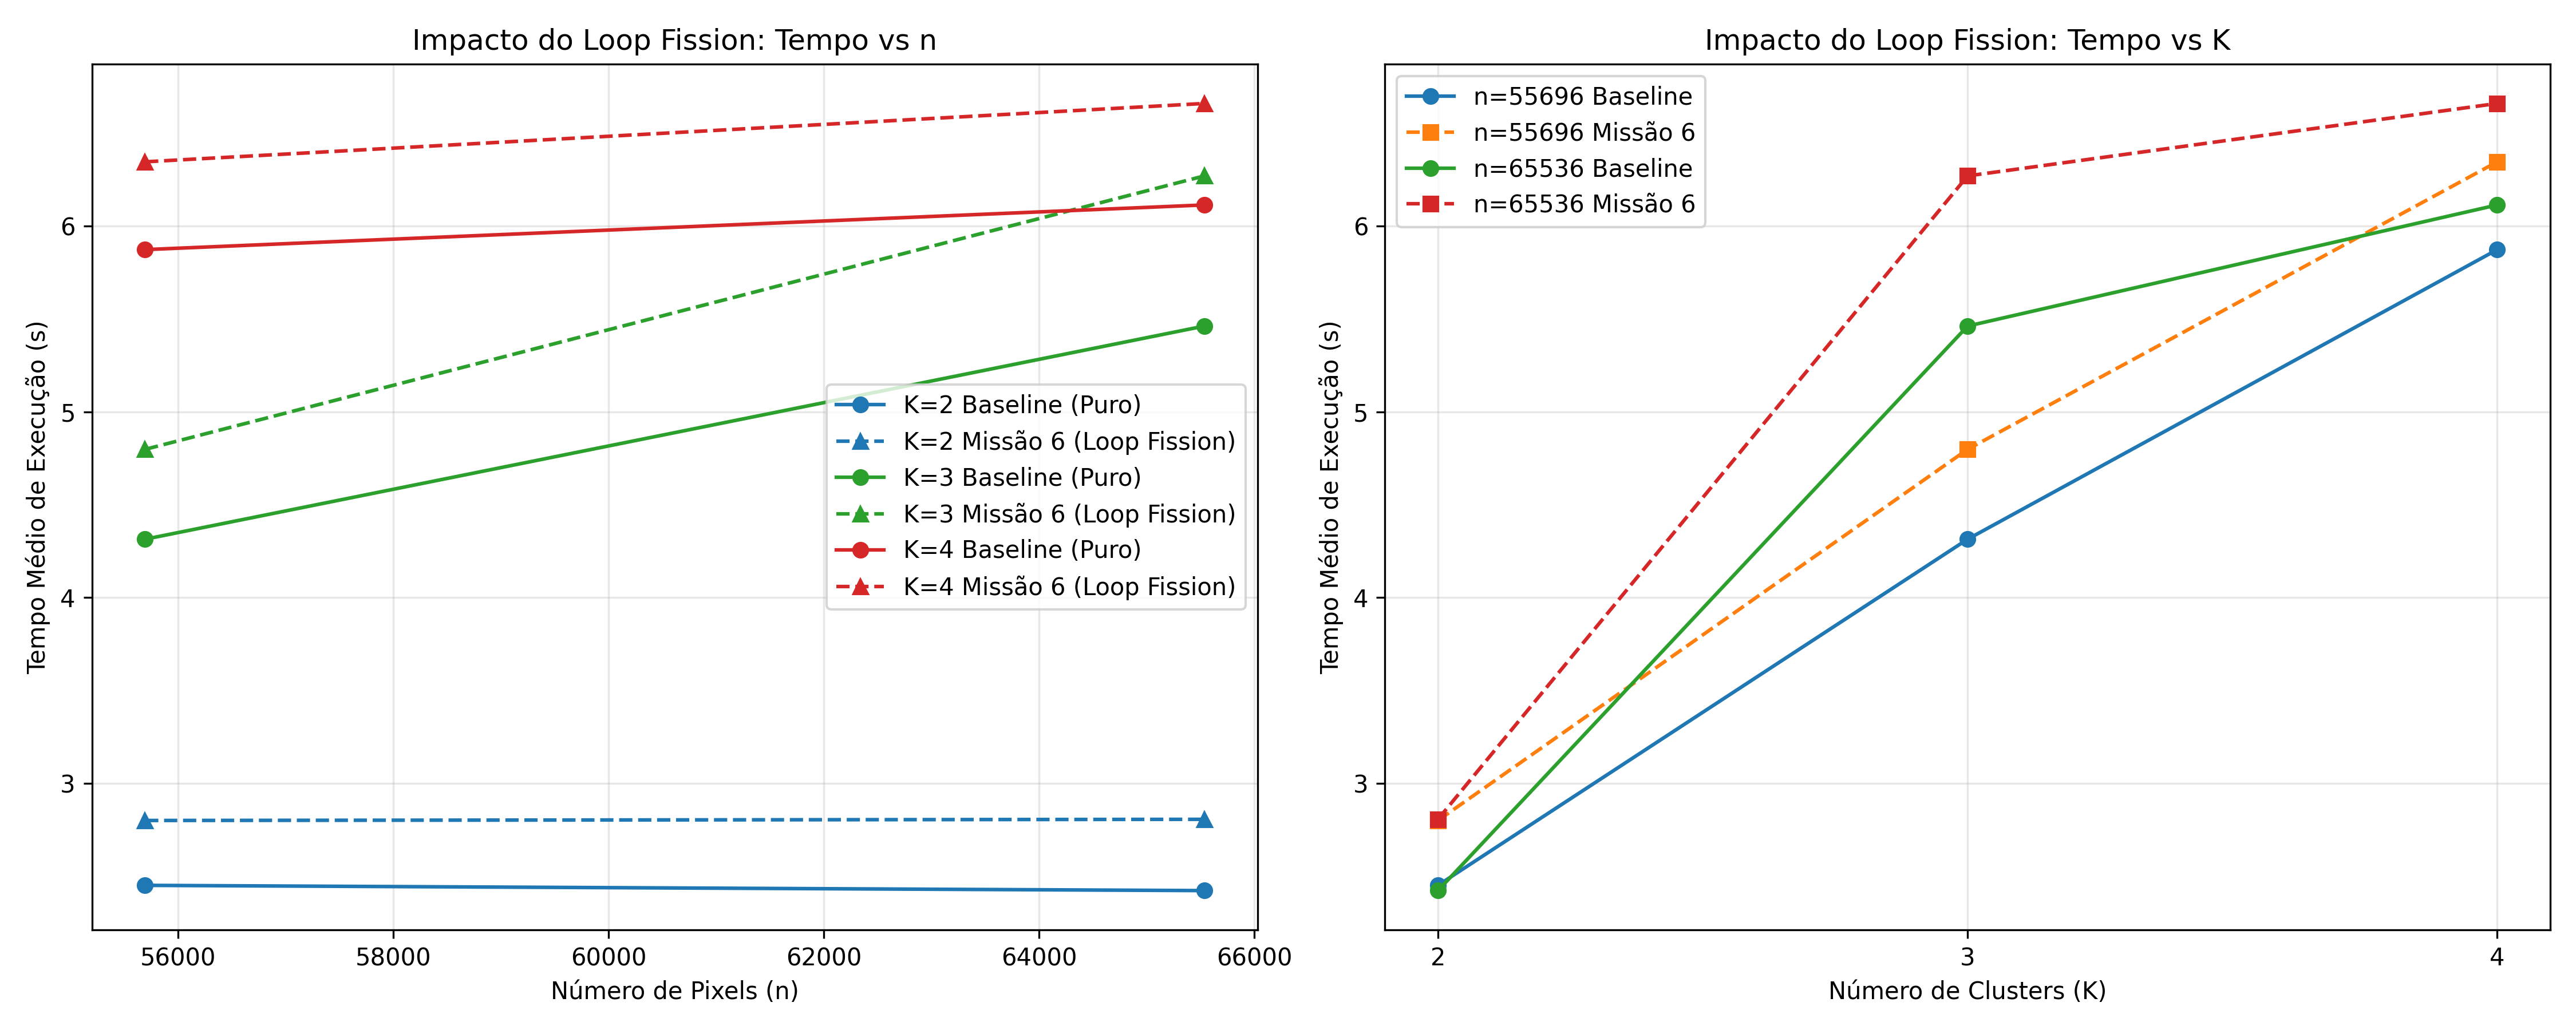
\includegraphics[width=0.92\textwidth]{segunda_unidade/resultados_missao_6/relatorio_comparativo_baseline_vs_missao6.png}
\caption{Cortes bidimensionais comparativos ($T$ vs $n$ e $T$ vs $K$) confrontando as medi\c{c}\~{o}es emp\'{i}ricas do Baseline e da Miss\~{a}o 6 (Loop Fission).}
\label{fig:comparativo2d}
\end{figure}

\begin{figure}[h!]
\centering
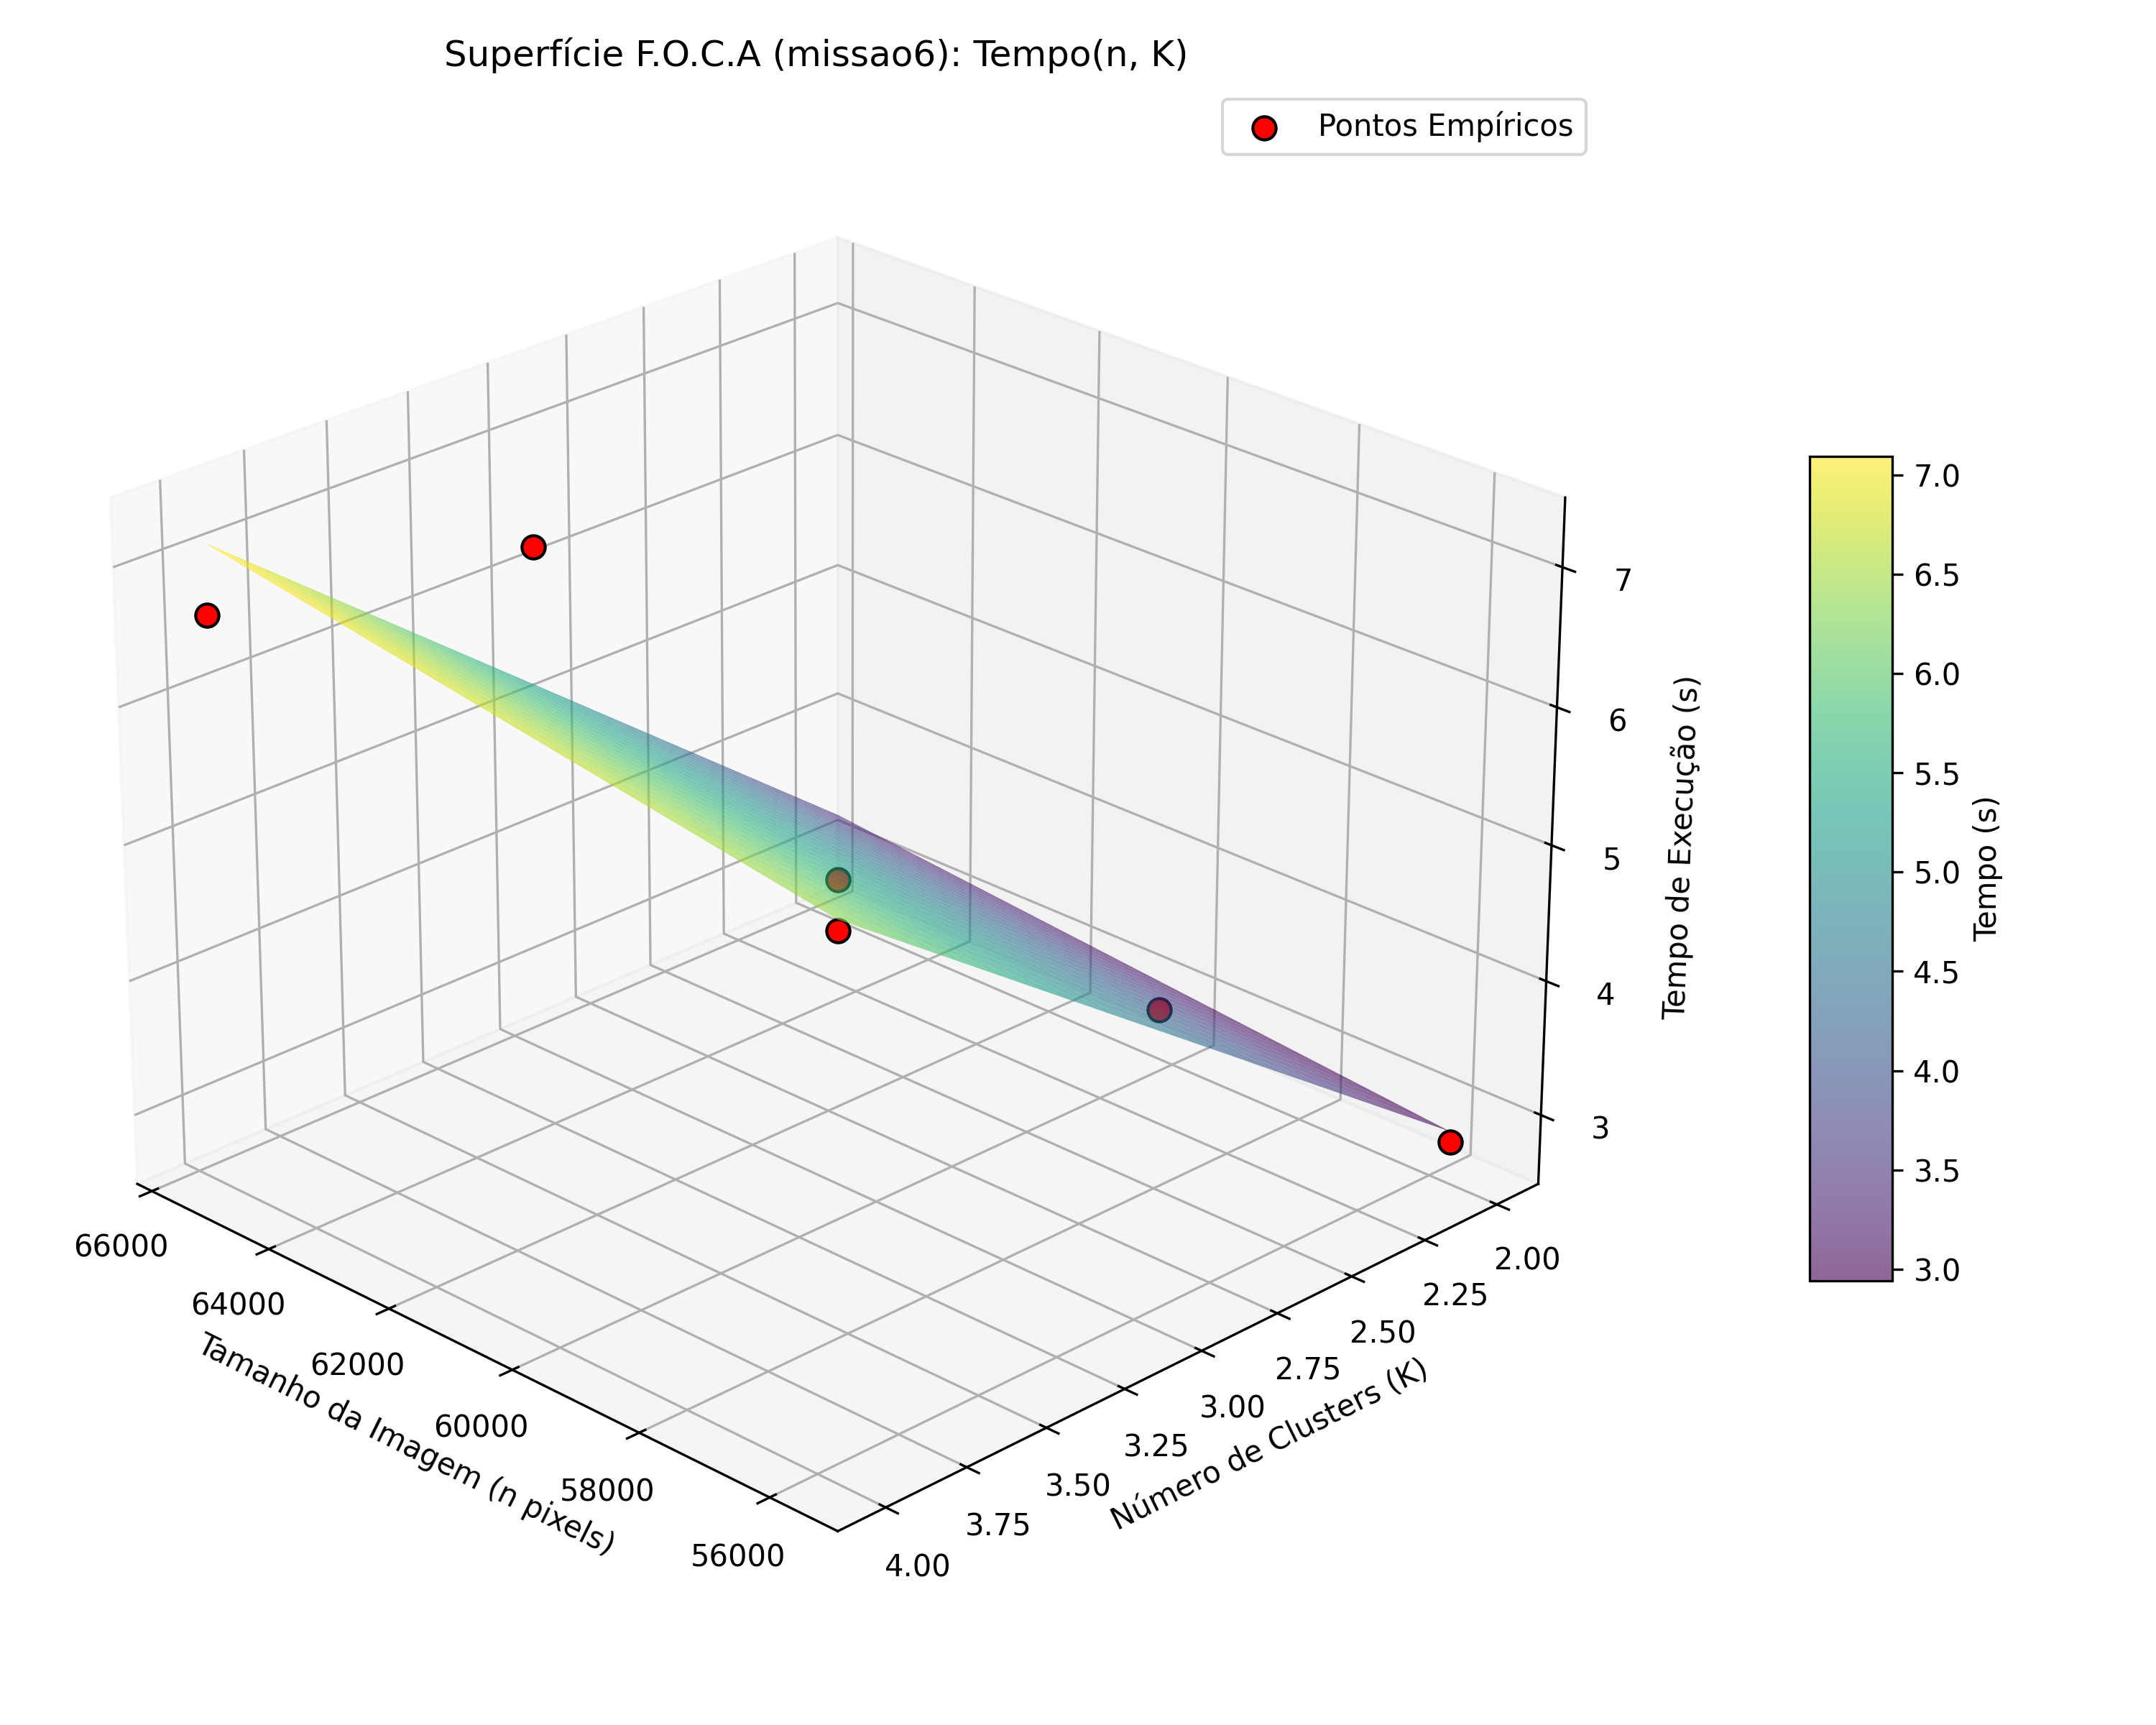
\includegraphics[width=0.75\textwidth]{segunda_unidade/resultados_missao_6/superficie_3d_foca.png}
\caption{Superf\'{i}cie tridimensional cont\'{i}nua calibrada $T_{\text{exp}}(n, K)$ projetada sobre os pontos emp\'{i}ricos coletados em bancada para a Miss\~{a}o 6.}
\label{fig:superficie3d}
\end{figure}

\end{document}
